\section{Translator}

We developed a tool to translate \conesc structures to plain nesC and compile
them into a binary. The translator performs two passes through the project, it
reads a \emph{Makefile} to get the main configuration component of the project
and briefly scans the components tree. During the second pass the tool performs
a deep analysis of each component and -- having the information about all
declared \emph{contexts} and \emph{context groups} -- generates nesC source
code. At the end of generation, our tool invokes nesC compiler and displays its
output. When compilation is finished, the tool removes generated files from the
file-system.

\putfigure{caption=\conesc translator diagram.,label=fig:ctd}{
 \centering
 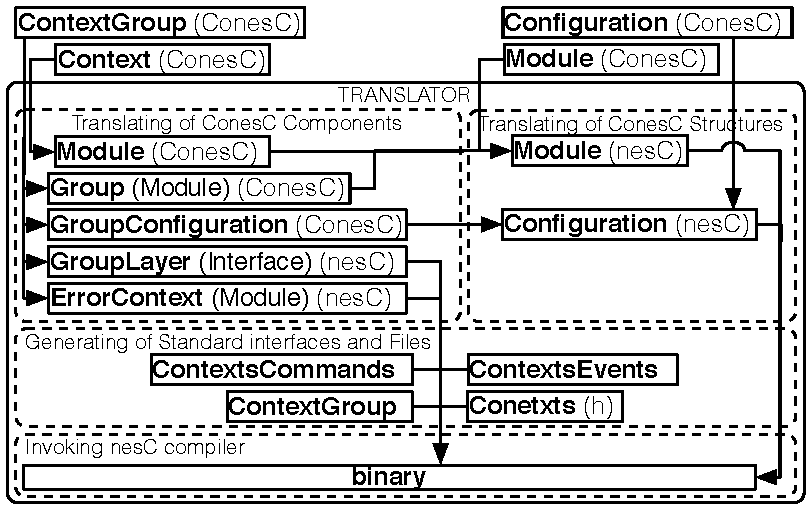
\includegraphics[width=\columnwidth]{pdf/translator}
}

The input of the translator contains of four types of components: context
configuration, context, module and configuration, as shown in
Fig.~\ref{fig:ctd}. The latter two possibly contain \conesc structures and do
not define the architecture of the project, while the former two are surely
written in \conesc and base a skeleton of software. Based on \emph{context
configuration} translator generates \emph{configuration} component -- a
description of the group, \emph{context group} module -- a wrapper and
controller of contexts, \emph{group layer} -- interface implemented by contexts,
and \emph{error context} module if it was not declared in the \emph{context
group}. \emph{Context} is translated into module by adding standard functions
and implementation of \emph{group layer} interface mentioned above.

After translating \emph{context groups} and \emph{contexts}, the tool handles
modules and configuration provided by a programmer and generated at the previous
stage, since the latter also may contain \conesc structures. Unlike the previous
stage, during this handling the tool just translates \conesc structures within
the functions written by a programmer without generation additional source code
based on them. The last preparation step is to generate standard files:
\emph{context commands} and \emph{context events} -- basic interfaces for
\emph{context} components, \emph{context group} -- basic interface for
\emph{context group} component, and \emph{Contexts.h} -- a definition of all the
contexts in the projects. The last step is invoking the nesC compiler to build a binary by using all the
generated and transformed components.
